\chapter{Customizing Tao}
\index{customizing}
\label{c:custom.tao}

\tao has been designed to be readily extensible with a minimum of
effort when certain rules are followed. 
This chapter discusses how this is done.

%----------------------------------------------------------------
\section{Initial Setup}
\label{s:cust.init}

Creating a custom version of \tao involves creating custom code that
is put in a directory that is distinct from the \vn{tao} directory that
contains the standard \tao code files. 

It is important to
remember that the code in the \vn{tao} directory is not to be modified.
This ensures that, as time goes on, and as \tao is developed by the 
"Taoist" developers, changes to the code in the \vn{tao} directories
will have a minimal chance to "break" your custom code.

To setup a custom \tao version do the following:
  \begin{enumerate}
  \item
Establish a base directory in which things will be
built. This directory can have any name.
Here we will call this directory \vn{ROOT}.
  \item
Make a subdirectory of \vn{ROOT} to put the code. 
This directory can have any name.
Here this directory will be called \vn{tao_custom}.
  \item
Copy the files from the directory \vn{tao/customization} to \vn{Root/tao_custom}. The
\vn{tao} directory is part of the \bmad package. If you do not know where to find it, ask
your local Guru where it is. Along with a \vn{README} file, there are two CMake script
files in the \vn{customization} directory:
\begin{example}
  CMakeLists.txt
  cmake.custom_tao
\end{example}
These scripts are setup to make an executable called \vn{custom_tao} but this can be
changed.
  \item
Copy the file \vn{tao/program/tao_program.f90} to \vn{ROOT/tao_custom}.
  \item
Copy as needed \vn{hook} files from \vn{tao/hook} to \vn{ROOT/tao_custom}. The hook files
you will need are the hook files you will want to modify to customize \tao. See below for
details. See \sref{s:cust.example} for an example.
  \item
Go to the \vn{ROOT/tao_custom} directory and use the command \vn{mk} to create the
executable \vn{ROOT/production/bin/custom_tao}. Similarly, the command \vn{mkd} will
create a debug executable \vn{ROOT/debug/bin/custom_tao}.
	\end{enumerate}

%----------------------------------------------------------------
\section{It's All a Matter of Hooks}
\index{customizing!hooks}

The golden rule when extending \tao is that you are only allowed to
customize routines that have the name ``hook'' in
them. These files are located in the directory \vn{tao/hook}.
To customize one of these files, copy it from \vn{tao/hook} to \vn{ROOT}
and then make modifications to the copy.

The reason for this golden rule is to ensure that, as time
goes by, and revisions are made to the \tao routines to extend it's
usefulness and to eliminate bugs, these changes will
have a minimum impact on the specialized routines you write.
What happens if the modification you want to do cannot be accomplished
by customizing a hook routine? The answer is to contact
the \tao programming team and we will modify \tao and provide the hooks 
you need so that you can then do your customization.

%----------------------------------------------------------------
\section{Initializing Hook Routines}

One way to initialize a hook routine is to read in parameters from an initialization file.
If an initialization file is used, the filename may be set using the
\vn{s%global%hook_init_file} string. This string may be set in the \vn{tao_params}
namelist (\sref{s:globals} or may be set on the command line using the
\vn{-hook_init_file} option (\sref{s:command.line}).

%----------------------------------------------------------------
\section{Hook Routines}

To get a good idea of how \tao works it is recommended to spend a
little bit of time going through the source files. This may also
provide pointers on how to make customizations in the hook routines. Of
particular interest is the module \vn{tao_lattice_calc_mod.f90} where tracking
and lattice parameters are computed. 

Plotting is based upon the \vn{quick_plot} subroutines which are
documented in the \bmad reference manual. If custom plotting is
desired this material should be reviewed to get familiar with the
concepts of ``graph'', ``box'', and ``page''.

The following is a run through of each of the hook routines. Each
routine is in a separate file called
\vn{tao/hook/<hook_routine_name>.f90}. See these files for subroutine
headers and plenty of comments throughout the dummy code to aid in the
modification of these subroutines.

%-----------------------------------------------------------------
\subsection{tao\_hook\_graph\_setup}
\index{customizing!tao_hook_graph_data_setup}

Use this to setup custom graph data for a plot.

%-----------------------------------------------------------------
\subsection{tao\_hook\_command}\index{customizing!tao_hook_commad}
\label{s:hook.command}

Any custom commands are placed here. The dummy subroutine already has
a bit of code that replicates what is performed in
\vn{tao_command}. Commands placed here are searched before the
standard \tao commands. This allows for the overwriting of any
standard \tao command.

By default, there is one command included in here: \vn{`hook'}. This
is just a simple command that doesn't really do anything and is for
the purposes of demonstrating how a custom command would be
implemented.

The only thing needed to be called at the end of a custom command is
\vn{tao_cmd_end_calc}. This will perform all of the steps listed in
Section~\sref{s:lat.calc}.

See Sec.~\sref{s:cust.read.example} for an example of how to use this hook.

%-----------------------------------------------------------------
\subsection{tao\_hook\_evaluate\_a\_datum}
\index{customizing!tao_hook_evaluate_a_datum}

Any custom data types are defined and calculated here. If a
non-standard data type is listed in the initialization files, then a
corresponding data type must be placed in this routine. The tutorial
uses this hook routine when calculating the emittance.

\tao evaluates data at each element while each lattice is being
calculated. At initialization time \tao determines which datums are to
be evaluated at each element then calls \vn{tao_evaluate_a_datum} at
each element for each datum that needs to be evaluated. If a range of
elements are specified for a datum then \vn{tao_evaluate_a_datum} is
called for this datum at the last element in the
range. \vn{tao_evaluate_a_datum} starts by calling
\vn{tao_hook_evaluate_a_datum} to evaluate the custom data types.

As explained in the dummy file, the datum merit type affects how a
datum's value should be calculated. There is a helper subroutine in
the dummy hook routine called \vn{load_it} to aid in modifying the
datum's value based on the merit type. If there is a range of elements
associated with datum then a merit type other than \vn{target}
requires that the entire range of elements associated with the datum
be searched for the appropriate value to be returned.  See
Chapter~\ref{c:opti} for details on the merit type.

For example, if the data type is \vn{orbit.x} (yes, this is already
defined in \tao) then the appropriate case item in
\vn{tao_hook_load_data_array} would be:
\begin{example}
select case (datum%data_type)

case ('orbit.x')
  call load_it (orb(:)%vec(1))
\end{example}
\vn{load_it} will then look at each datum. If the merit type is other
than \vn{target} then \vn{load_it} will search the appropriate range
of elements for either the minimum or maximum horizontal orbit value
and this will be the datum's value. Because, a datum may refer to a
range of elements, the entire orbit array (from 0 to \vn{n_ele_max})
is passed to \vn{load_it} for each \vn{orbit.x} datum.

If the only merit type that is going to be used is \vn{target} then
\vn{load_it} can be ignored.

%-----------------------------------------------------------------
\subsection{tao\_hook\_init1 and tao_hook_init2}
\label{s:hook.init}
\index{customizing!tao_hook_init}

After the \vn{design} lattice and the global and universe structures are initialized,
\vn{tao_hook_init1} is called from the \vn{tao_init} routine. Here, any further
initializations can be added. In particular, if any custom hook structures need to be
initialized, here's the place to do it. 

Further down in \vn{tao_init}, \vn{tao_hook_init2} is called. Normally you will want to
use \vn{tao_hook_init1}. However, \vn{tao_hook_init2} can be used, for example, ! to set
model variable values different from design variable values since when \vn{tao_hook_init1}
is called the \vn{model} lattice has not yet been initialized.

%-----------------------------------------------------------------
\subsection{tao\_hook\_init\_design\_lattice}
\index{customizing!tao_hook_init_design_lattice}

This will do a custom lattice initialization. The standard lattice
initialization just calls \vn{bmad_parser} or \vn{xsif_parser}. If
anything more complex needs to be done then do it here. This is also
where any custom overlays or other elements would be inserted after
the parsing is complete. But in general, anything placed here should,
in principle, be something that can be placed in a lattice file.

\textbf{This is the only routine that should insert elements in the
ring}. This is because the \tao data structures use the element index
for each element associated with the datum. If all the element indexes
shift then the data structures will break. If new elements need to be
inserted then modify this routine and recompile. You can alternatively
create a custom initialization file used by this routine that reads in
any elements to be inserted.

%-----------------------------------------------------------------
\subsection{tao\_hook\_lattice\_calc}
\index{customizing!tao_hook_lattice_calc}

The standard lattice calculation can be performed for single particle,
particle beam tracking and will recalculate the
orbit, transfer matrices, twiss parameters and load the data
arrays. If something else needs to be performed whenever the lattice
is recalculated then it is placed here. A custom lattice calculation
can be performed on any lattice separately, this allows for the
possibility of, for example, tracking a single particle for one
lattice and beams in another.

%-----------------------------------------------------------------
\subsection{tao\_hook\_merit\_data}
\index{customizing!tao_hook_merit_data}

A custom data merit type can be defined here. Table~\ref{t:con.type}
lists the standard merit types. If a custom merit type is used then
\vn{load_it} in \vn{tao_hook_load_data_array} may also need to be
modified to handle this merit type, additionally, all standard data
types may need to be overridden in \vn{tao_hook_load_data_array} in
order for the custom \vn{load_it} to be used.  See
\vn{tao_merit.f90} for how the standard merit types are
calculated.

%-----------------------------------------------------------------
\subsection{tao\_hook\_merit\_var}
\index{customizing!tao_hook_merit_var}

This hook will allow for a custom variable merit type. However, since
there is no corresponding data transfer, no \vn{load_it} routine needs
to be modified.  See \vn{tao_merit.f90} for how the standard
merit types are calculated.

%-----------------------------------------------------------------
\subsection{tao\_hook\_optimizer}
\index{customizing!tao_hook_optimizer}

If a non standard optimizer is needed, then it can be implemented
here. See the \vn{tao_*_optimizer.f90} files for how the
standard optimizers are implemented.

%-----------------------------------------------------------------
\subsection{tao\_hook\_plot\_graph}
\index{customizing!tao_hook_plot_graph}

This will customize the plotting of a graph. See the \tao module
\vn{tao_plot_mod} for details on what it normally done. You will also
need to know how \vn{quick_plot} works (See the \bmad manual).

%-----------------------------------------------------------------
\subsection{tao\_hook\_plot\_data\_setup}
\index{customizing!tao_hook_plot_data_setup}

Use this routine to override the \vn{tao_plot_data_setup} routine which
essentially transfers the information from the \vn{s%u(:)%data} arrays
to the \vn{s%plot_page%region(:)%plot%graph(:)%curve(:)} arrays. This
may be useful if you want to make a plot that isn't simply the
information in a data or variable array.

%-----------------------------------------------------------------
\subsection{tao\_hook\_post\_process\_data}
\index{customizing!tao_hook_post_process_data}

Here can be placed anything that needs to be done after the data
arrays are loaded. This routine is called immediately after the data
arrays are called and before the optimizer or plotting is done, so any
final modifications to the lattice or data can be performed here.

%-----------------------------------------------------------------
%\chapter{Plotting}
%\label{s:prog.plotting} 

%\fbox{this chapter is yet to be completed!} 

%----------------------------------------------------------------
\section{Adding a New Data Type Example}
\label{s:cust.example}

As an example of a customization, let's include a new data type called
\vn{particle_emittance}. This will be the non-normalized x and y
emittance as found from the Courant-Snyder invariant. This data type
will behave just like any other data type (i.e.  \vn{orbit},
\vn{phase} etc...). 

This example will only require the modification of one file:
\vn{tao_hook_evaluate_a_datum.f90}. This file should be copied
from the \vn{tao/hook} directory and put in your \vn{ROOT/code}
directory (\sref{s:cust.init}).

The formula for single particle emittance is
\Begineq
  \epsilon = \gamma x^{2} + 2 \alpha x x' + \beta x'^{2}
  \label{e:emittance}
\Endeq
Place the following code in \vn{tao_hook_evaluate_a_datum.f90} in the
\cmd{case select} construct (also add the necessary type declarations)
\begin{verbatim}
  case ('particle_emittance.x') 

    datum_value =  ( ele%x%gamma * tao_lat%orb(ix1)%vec(1)**2 + &
		     2 * ele%x%alpha * tao_lat%orb(ix1)%vec(1) * tao_lat%orb(ix1)%vec(2) + &
		     ele%x%beta * tao_lat%orb(ix1)%vec(2)**2)
    
  case ('particle_emittance.y')

    datum_value = ( ele%y%gamma * tao_lat%orb(ix1)%vec(3)**2 + &
		     2 * ele%y%alpha * tao_lat%orb(ix1)%vec(3) * tao_lat%orb(ix1)%vec(4) + &
		     ele%y%beta * tao_lat%orb(ix1)%vec(4)**2)
\end{verbatim}
This defines what is to be calculated for each \vn{particle_emittance}
datum.  There are two transverse coordinates, so two definitions need
to be made, one for each dimension.

Now you just need to declare the data types in the \cmd{tao.init} and
\cmd{tao_plot.init} files. For the sake of this example, modify the
example files found in the \vn{tao/example} directory
\begin{example}
	mkdir ROOT/my_example
  cp tao/example/*.init ROOT/my_example
  cp tao/example/*.lat ROOT/my_example
\end{example}

In \cmd{ROOT/my_example/tao.init} add the following lines to the data
declarations section
\begin{example}
  &tao_d2_data
    d2_data%name = "particle_emittance" 
    universe = 0 
    n_d1_data = 2
  /

  &tao_d1_data
    ix_d1_data = 1
    d1_data%name = "x"  
    default_weight = 1
    use_same_lat_eles_as = 'orbit.x"
  /

  &tao_d1_data
    ix_d1_data = 2
    d1_data%name = "y"  
    default_weight = 1
    use_same_lat_eles_as = 'orbit.x"
  /
\end{example}

In \cmd{ROOT/my_example/tao_plot.init} add the following lines to the end
of the file
\begin{example}
  &tao_template_plot
    plot%name = 'particle_emittance'
    plot%x%min =   0
    plot%x%max = 100
    plot%x%major_div = 10
    plot%x%label = ' '
    plot%x_axis_type = 'index'
    plot%n_graph = 2
  /
  
  &tao_template_graph
    graph%name = 'x'
    graph_index = 1
    graph%box = 1, 2, 1, 2
    graph%title = 'Horizontal Emittance (microns)'
    graph%margin =  0.15, 0.06, 0.12, 0.12, '%BOX'
    graph%y%label = 'x'
    graph%y%max =  15
    graph%y%min =  0.0
    graph%y%major_div = 4
    graph%n_curve = 1
    curve(1)%data_source = 'data'
    curve(1)%data_type   = 'particle_emittance.x'
    curve(1)%y_axis_scale_factor = 1e6 !convert from meters to microns
  /

  &tao_template_graph
    graph%name = 'y'
    graph_index = 2
    graph%box = 1, 1, 1, 2
    graph%title = 'Vertical Emittance (microns)'
    graph%margin =  0.15, 0.06, 0.12, 0.12, '%BOX'
    graph%y%label = 'Y'
    graph%y%max =  15
    graph%y%min =  0.0
    graph%y%major_div = 4
    graph%n_curve = 1
    curve(1)%data_source = 'data'
    curve(1)%data_type = 'particle_emittance.y'
    curve(1)%units_factor = 1e6 !convert from meters to microns
  /
\end{example}
These namelists are described in detail in Chapter~\ref{c:init}.

We are now ready to compile and then run the program. The \tao library
should have already been created so all you need to do is
\begin{example}
	cd ROOT/code
	mk
  cd ROOT/my_example
  ../production/bin/custom_tao
\end{example}

After your custom \tao initializes type
\begin{example}
  place bottom particle_emittance
  scale
\end{example}
Your plot should look like Figure~\ref{f:plot.emittance}.

The emittance (as calculated) is not constant. This is due to
dispersion and coupling throughout the ring. \bmad provides a routine
to find the particle emittance from the twiss parameters that includes
dispersion and coupling called \vn{orbit_amplitude_calc}.

\begin{figure}
  \centering
  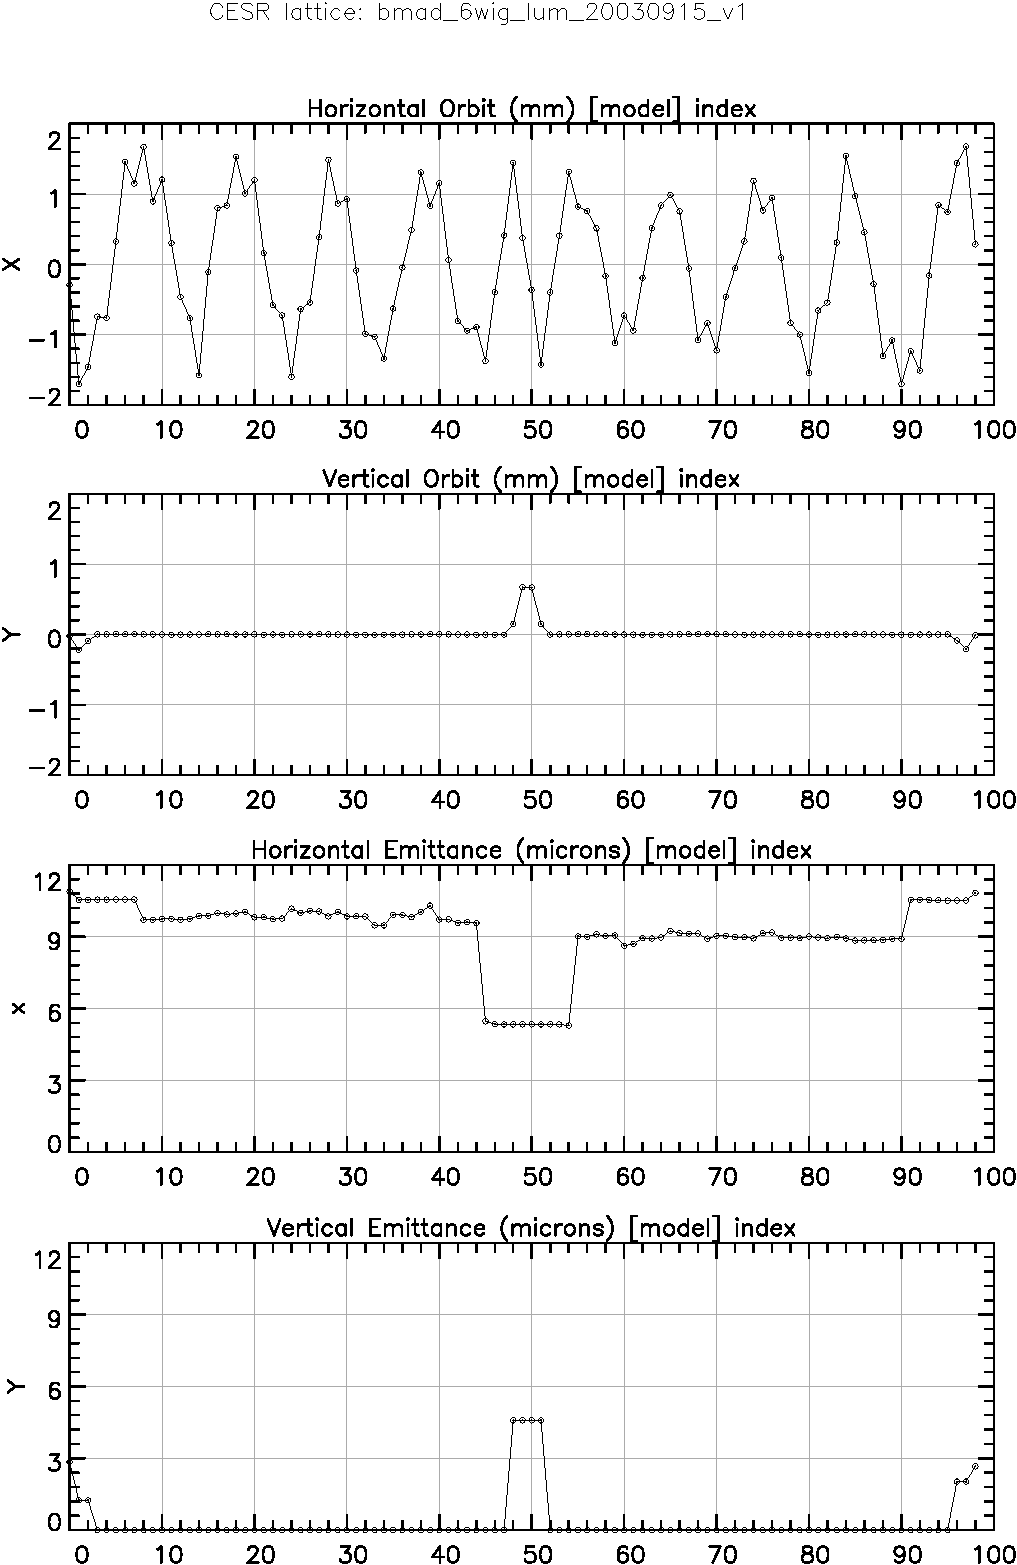
\includegraphics[width=5in]{plot-emittance.pdf}
  \caption{Custom data type: non-normalized emittance}
  \label{f:plot.emittance}
\end{figure}

%----------------------------------------------------------------
\section{Reading in Measured Data Example}
\label{s:cust.read.example}

This section shows how to construct a customized version of \tao, called \vn{ping_tao}, to
read in measured data for analysis. This example uses data from the Fermilab proton
recirculation. The data is obtained by measuring the orbit turn-by-turn of a beam that has been
initially pinged to give it a finite oscillation amplitude.

The files for constructing \vn{ping_tao} can be found
in the directory
\begin{example}
  tao/examples/custom_tao_with_measured_data
\end{example}
The files in this directory are as follows:
\begin{description}
  \item[CMakeLists.txt, cmake.ping_tao] \Newline
Script files for creating \vn{ping_tao}. See Sec.~\sref{s:cust.init}.
  \item[README] \Newline
The \vn{README} file gives some instructions on how to create \vn{ping_tao}
  \item[RRNOVAMU2E11172016.bmad] \Newline
Lattice file for the proton recirculation ring.
  \item[data] \Newline
Directory where some ping data is stored
  \item[tao.init] \Newline
\tao initialization file defining the appropriate data and variable structures (\sref{s:init.global})
  \item[tao.startup] \Newline
File with some command that are executed when \tao is started. These commands will read in
and plot some data.
  \item[tao_hook_command.f90] \Newline
Custom code for reading in ping data. The template used to construct this file is at
\vn{tao/hook/tao_hook_command.f90} (\sref{s:hook.command}).
  \item[tao_plot.init] \Newline
File for defining plot parameters (\sref{s:init.plot}).
  \item[tao_program.f90] \Newline
copy of the \vn{tao/program/tao_program.f90} file (\sref{s:cust.init}).
\end{description}

After creating the \vn{ping_tao} program (see the \vn{README} file), the program can
be run by going to the custom_tao_with_measured_data directory and using the command:
\begin{example}
	../production/bin/ping_tao
\end{example}

The customized \vn{tao_hook_command} routine implements a custom command called
\vn{pingread}.  This command will read in ping data. Ping data is the amplitude and phase
of the beam oscillations at a BPM for either the \vn{a-mode} or \vn{b-mode} oscillations.
See the write up on ping data types in Sec.~\sref{s:data.types} under \vn{ping_a.amp_x},
and \vn{ping_b.amp_x} for more details.

The data files in the \vn{data} directory contain data for either the \vn{a-mode} or \vn{b-mode} ping at either
the horizontal or vertical BPMs.

The syntax of the \vn{pingread} command is:
\begin{example}
  pingread <mode> <filename> <data_or_ref>
\end{example}
The first argument, \vn{<mode>}, should be either ``\vn{a_mode}'' ``\vn{b_mode}''
indicating wether the data is for the \vn{a-mode} \vn{b-mode} analysis (a better setup
would encode this information in the data file itself). The second argument, \vn{filename}
is the name of the data file, and the third argument, \vn{data_or_ref} should be
``\vn{data}'' or ``\vn{reference}'' indicating that the data is to be read into the
\vn{meas_value} or \vn{ref_value} of the appropriate \vn{tao_data_struct}.

%----------------------------------------------------------------
\subsection{Analysis of the tao\_hook\_command.f90 File}
\label{s:hook.cmd.anal}

The first part of the \vn{tao_hook_command} routine parses the command line to see
if the \vn{pingread} command is present. The relevant code, somewhat condensed, is:
\begin{example}
  subroutine tao_hook_command (command_line, found)

  !!!! put your list of hook commands in here. 

  character(16) :: cmd_names(1) = [character(16):: 'pingread']  

  ! "found" will be set to TRUE if the command is found.

  found = .false.

  ! strip the command line of comments

  call string_trim (command_line, cmd_line, ix_line)
  ix = index(cmd_line, '!')
  if (ix /= 0) cmd_line = cmd_line(:ix-1)        ! strip off comments

  ! blank line => nothing to do

  if (cmd_line(1:1) == '') return

  ! match first word to a command name
  ! If not found then found = .false.

  call match_word (cmd_line(:ix_line), cmd_names, ix_cmd, .true., .true., cmd_name)
  if (ix_cmd < 0) then
    call out_io (s_error$, r_name, 'AMBIGUOUS HOOK COMMAND')
    found = .true.
    return
  endif

  found = .true.
  call string_trim (cmd_line(ix_line+1:), cmd_line, ix_line)
\end{example}

Note: To quickly find information on routines and structures, use the \vn{getf} and \vn{listf}
scripts as explained in the \bmad manual. For example, typing ``\vn{getf string_trim}'' 
on the system command line will give information on the string_trim subroutine.

The above code tests to see if the command is \vn{pingread} and, if not, returns without
doing anything.

If the \vn{pingread} command is found, the rest of the command line is parsed to get the 
\vn{<mode>}, \vn{<filename>}, and \vn{<data_or_ref>} arguments.

In the \vn{tao.init} file, a \vn{tune} d2 datum is setup to have two \vn{d1} datum arrays
One for the \vn{a}-mode tune and one for the \vn{b}-mode tune:
\begin{example}
  \&tao_d2_data
    d2_data%name = "tune"
    universe = '*'  ! apply to all universes
    n_d1_data = 2
  /

  \&tao_d1_data
    ix_d1_data = 1
    d1_data%name = "a"
    default_weight = 1e6
    ix_min_data = 1
    ix_max_data = 1
  /

  \&tao_d1_data
    ix_d1_data = 2
    d1_data%name = "b"
    default_weight = 1e6
    ix_min_data = 1
    ix_max_data = 1
  /
\end{example}
And each \vn{d1} array has only one datum since the \vn{a}-mode and \vn{b}-mode tunes have
only one value associated with them (as opposed to, say an orbit which will have multiple
values from different BPMs).

In a data file there is a header section which, among other things, records the tune.
In a line beginning with the word ``\vn{Tune}''. Example:
\begin{example}
                   Horz         Vert         Sync.                           
   Tune           ( .452444)   ( .404434)   ( 0      ) 2p                    
\end{example}

In the \vn{tao_hook_command} file, after the arguments are parsed, the header part of the
data file is read to extract the tune datums:
\begin{example}
  type (tao_d2_data_array_struct), allocatable :: d2(:)
  ...
  if (line(1:4) == 'Tune') then
    call tao_find_data (err, 'tune', d2_array = d2)
    if (size(d2) /= 1) then
      call out_io (s_fatal$, r_name, 'NO TUNE D2 DATA STRUCTURE DEFINED!')
      return
    endif
\end{example}
The call to \vn{tao_find_data} looks for a \vn{d2} data structure named \vn{tune}. This
structure is setup in the \vn{tao.init} file. Alternatively, the \vn{ping_tao} program
could be configured to automatically setup the appropriate data and/or variable structures
via the \vn{tao_hook_init1} routine (\sref{s:hook.init}). 

The returned value from the call to \vn{tao_find_data} is an array called \vn{d2} of type
\vn{tao_d2_data_array_struct}. \vn{d2} holds an array of pointers to all
\vn{d2_data_struct} structures it can find. In general, there could be multiple such
structures if multiple universes are being used or if the match string, in this case
\vn{'tune'}, contained wild card characters. In this case, the expectation is that there
will only one universe used and thus there should be one and only one structure that
matches the name \vn{tune}. This structure will be pointed to by \vn{d2(1)%d2}. The
appropriate datums, will be:
\begin{example}
  d2(1)%d2%d1(1)%d(1)   ! a-mode tune
  d2(1)%d2%d1(1)%d(2)   ! b-mode tune
\end{example}
The values read from the data file are put in these datums via the code:
\begin{example}
  if (data_or_ref == 'data') then
    d2(1)%d2%d1(1)%d(1)%meas_value = twopi * (data_tune_a + nint(design_tune_a))
    d2(1)%d2%d1(1)%d(1)%good_meas = .true.
    d2(1)%d2%d1(2)%d(1)%meas_value = twopi * (data_tune_b + nint(design_tune_b))
    d2(1)%d2%d1(2)%d(1)%good_meas = .true.
  else
    d2(1)%d2%d1(1)%d(1)%ref_value = twopi * (data_tune_a + nint(design_tune_a))
    d2(1)%d2%d1(1)%d(1)%good_ref = .true.
    d2(1)%d2%d1(2)%d(1)%ref_value = twopi * (data_tune_b + nint(design_tune_b))
    d2(1)%d2%d1(2)%d(1)%good_ref = .true.
  endif      
\end{example}

The next step is to setup pointers to the appropriate data arrays to receive the ping data.
In the data file the ping data looks like:
\begin{example}
  BPM           Phase    Ampl.   RMSdev     Beta  bml_psi *Calib Old_Cal     
  R:HP222    -0.27314  0.46085    0.078    1.863  0.35183                         
  R:HP224    -0.05939  0.28277    0.143    0.701 -0.43442                         
  R:HP226     0.23140  0.31712    0.075    0.882 -0.14363                         
  ... etc ...
\end{example}
The ``\vn{H}'' in \vn{R:HP222}, etc. indicates that the data is from BPMs that only
measure the horizontal displacement of the beam. Alternatively, a ``\vn{V}'' would
indicate data from vertical measurement BPMs.

In the \vn{tao_hook_command} file the data pointers are setup by the code:
\begin{example}
  type (tao_d1_data_array_struct), allocatable, target :: d1_amp_arr(:), d1_phase_arr(:)
  ...
  if (line(3:3) == 'H') then
    if (mode == 'a_mode') then
      call tao_find_data (err, 'ping_a.amp_x', d1_array = d1_amp_arr)
      call tao_find_data (err, 'ping_a.phase_x', d1_array = d1_phase_arr)
    else 
      call tao_find_data (err, 'ping_b.amp_x', d1_array = d1_amp_arr)
      call tao_find_data (err, 'ping_b.phase_x', d1_array = d1_phase_arr)
    endif
  elseif (line(3:3) == 'V') then
    if (mode == 'a_mode') then
      call tao_find_data (err, 'ping_a.amp_y', d1_array = d1_amp_arr)
      call tao_find_data (err, 'ping_a.phase_y', d1_array = d1_phase_arr)
    else 
      call tao_find_data (err, 'ping_b.amp_y', d1_array = d1_amp_arr)
      call tao_find_data (err, 'ping_b.phase_y', d1_array = d1_phase_arr)
    endif
\end{example}
\vn{line(3:3)} is either \vn{H} or \vn{V} indicating horizontal or vertical orbit
measuring BPMs. In this case, the call to the \vn{tao_find_data} routine returns \vn{d1}
data arrays to the amplitude data (\vn{d1_amp_arr}) and phase data (\vn{d1_phase_arr}).
Just like the tune data, since it is assumed only one universe is being used, there should
be one and only \vn{d1} structure for the phase and only one \vn{d1} structure for the amplitude:
\begin{example}
  d1_amp_arr(1)%d1      ! d1 struucture for the amplitude data
  d1_phase_arr(1)%d1    ! d1 struucture for the phase data
\end{example}
To save on typing, and make the code clearer, pointers are used to point to these structures:
\begin{example}
  type (tao_d1_data_struct), pointer :: d1_phase, d1_amp
  ...
  d1_amp => d1_amp_arr(1)%d1
  d1_phase => d1_phase_arr(1)%d1
\end{example}
The array of datums for the amplitude and phase data will be \vn{d1_amp%d(:)} and
\vn{d1_phase%d(:)} respectively.

After the \vn{d1_amp} and \vn{d1_phase} pointers have been set, there is a loop over all
the lines in the file to extract the ping data. One problem faced is that the order of the
data in the file is not the same as the order of the data in \vn{d1} structures.  [The
data in the file is sorded in increasing numberical order in the BPM name while the order
in the \vn{d1} structures is sorted by increasing logitudinal s-position.]  To get around
this problem, the BPM name in the file is used to locate the appropriate datum (the
associated BPM element name is stored in the \vn{%ele_name} component of the datums):
\begin{example}
  character(140) :: cmd_word(12), ele_name
  ... 
  call tao_cmd_split (line, 4, cmd_word, .false., err)
  read (cmd_word(2), *) r1
  read (cmd_word(3), *) r2
  ele_name = cmd_word(1)
  datum_amp => tao_pointer_to_datum(d1_amp, ele_name(3:))
  datum_phase => tao_pointer_to_datum(d1_phase, ele_name(3:))
\end{example}
The \vn{line} string holds a line from the data file, the call to \vn{tao_cmd_split}
splits the line into word chunks and puts them into the array \vn{cmd_word(:)}.
\vn{cmd_word(1)} holds the first word which is the BPM name with ``\vn{R:}'' prepended to
the name. The calls to \vn{tao_pointer_to_datum} return pointers, \vn{datum_amp} and
\vn{datum_phase}, to the approbriate datums given the BPM name. 

After the appropriate datums have been identified, the ping data values read from the data
file, \vn{r1} and \vn{r2}, are used to set the appropriate components:
\begin{example}
  if (data_or_ref == 'data') then
    datum_phase%good_meas = .true.
    datum_amp%meas_value = r2
    datum_amp%good_meas = .true.
  else
    datum_phase%good_ref = .true.
    datum_amp%ref_value = r2
    datum_amp%good_ref = .true.
  endif
\end{example}

One problem is that individual data phase data points can be off by factors of $2\pi$. To
correct this, the measured phase values are shifted by factors of $2\pi$ so that they are
within $\pm\pi$ of the design values. There is an added ``branch cut'' problem here in
that, even without the factors of $2\pi$ problem, the measured phases will be off from the
design values by some arbitrary amount (determined by how the zero phase is defined in the
program that created the data file). If this difference between the zero phase of the data
and the zero phase of design lattice (in the design lattice, the phase is taken to be zero
at the beginning of the lattice) is close enough to $\pi$, the shifting of the phases by
factors of $2\pi$ will not be correct. For this reason, a best guess as to what the offset
is is used in the calculation to avoid the branch cut problem:
\begin{example}
  rms_best = 1e30

  do i = 1, 20
    offset = i / 20.0
    data = data + nint(design + offset - data)
    rms = sum((data - design - offset)**2, mask = ok)
    if (rms < rms_best) then
      offset_best = offset
      rms_best = rms
    endif
  enddo

  data = data + nint(design + offset_best - data)
\end{example}
